\documentclass[aspectratio=169]{beamer}
% Shared Beamer setup for Fall 2026 course slides.
\mode<presentation>{
  \usetheme{Madrid}
  \usecolortheme{default}
}

\definecolor{CalPolyGreen}{HTML}{154734}
\definecolor{CalPolyGold}{HTML}{BD8B13}
\definecolor{DeckInk}{HTML}{1F2933}
\definecolor{DeckMuted}{HTML}{5F6B7A}

\setbeamercolor{structure}{fg=CalPolyGreen}
\setbeamercolor{palette primary}{bg=CalPolyGreen,fg=white}
\setbeamercolor{palette secondary}{bg=DeckInk,fg=white}
\setbeamercolor{palette tertiary}{bg=CalPolyGold,fg=DeckInk}
\setbeamercolor{frametitle}{bg=CalPolyGreen,fg=white}
\setbeamercolor{title}{fg=CalPolyGreen}
\setbeamercolor{normal text}{fg=DeckInk,bg=white}
\setbeamercolor{block title}{bg=CalPolyGreen,fg=white}
\setbeamercolor{block body}{bg=black!3,fg=DeckInk}

\setbeamertemplate{navigation symbols}{}
\setbeamertemplate{footline}[frame number]
\setbeamertemplate{itemize item}{\color{CalPolyGold}$\blacktriangleright$}
\setbeamertemplate{itemize subitem}{\color{CalPolyGreen}$\bullet$}

\newcommand{\CourseNumber}{Course}
\newcommand{\CourseTitle}{Course Title}
\newcommand{\LectureNumber}{0}
\newcommand{\LectureTitle}{Lecture Title}
\newcommand{\LectureDate}{Date}
\newcommand{\CourseUnit}{Unit}

\newcommand{\coursenumber}[1]{\renewcommand{\CourseNumber}{#1}}
\newcommand{\coursetitle}[1]{\renewcommand{\CourseTitle}{#1}}
\newcommand{\lecturenumber}[1]{\renewcommand{\LectureNumber}{#1}}
\newcommand{\lecturetitle}[1]{\renewcommand{\LectureTitle}{#1}}
\newcommand{\lecturedate}[1]{\renewcommand{\LectureDate}{#1}}
\newcommand{\courseunit}[1]{\renewcommand{\CourseUnit}{#1}}

\author{Kirk Duran}
\institute{California Polytechnic State University, San Luis Obispo}
\date{\LectureDate}

\newcommand{\makedecktitle}{
  \begin{frame}[plain]
    \vspace{0.25in}
    {\usebeamerfont{title}\color{CalPolyGreen}\LectureTitle\par}
    \vspace{0.18in}
    {\large \CourseNumber{}: \CourseTitle\par}
    \vspace{0.08in}
    {\large Lecture \LectureNumber{} -- \LectureDate\par}
    \vfill
    {\small Kirk Duran \textbar{} Cal Poly, San Luis Obispo\par}
  \end{frame}
}

\newcommand{\placeholdernote}{
  \begin{block}{Placeholder}
    Replace these bullets with the final lecture material, examples, and in-class activities.
  \end{block}
}

\AtBeginSection[]{
  \begin{frame}{Roadmap}
    \tableofcontents[currentsection]
  \end{frame}
}

\graphicspath{{../assets/lecture-01/}}

\newcommand{\portraitcard}[3]{%
  \begin{minipage}[t]{0.235\linewidth}
    \centering
    \IfFileExists{../assets/lecture-01/#1}{%
      \includegraphics[width=\linewidth,height=1.0in,keepaspectratio]{#1}%
    }{%
      \fcolorbox{CalPolySage}{CalPolyBeige}{%
        \parbox[c][0.9in][c]{0.88\linewidth}{\centering\scriptsize Portrait pending}%
      }%
    }%
    \vspace{0.04in}

    {\bfseries\scriptsize #2\par}
    {\scriptsize #3\par}
  \end{minipage}%
}

\coursenumber{CS 1001}
\coursetitle{Introduction to Computing}
\lecturenumber{1}
\lecturetitle{Introduction to Computing}
\lecturedate{August 24, 2026}
\courseunit{1. Computing and Program Execution}

\begin{document}

\makedecktitle

\begin{frame}[shrink=3]{Welcome}
  \begin{columns}[T,onlytextwidth]
    \begin{column}{0.48\textwidth}
      \begin{keyidea}
        This course is about learning how computation works, and how to use it to solve problems.
      \end{keyidea}
      \begin{itemize}
        \item Instructor: Kirk Duran
        \item Course: \CourseNumber, \CourseTitle
        \item Unit: \CourseUnit
        \item Slides, examples, and assignments will live on Canvas.
      \end{itemize}
    \end{column}
    \begin{column}{0.47\textwidth}
      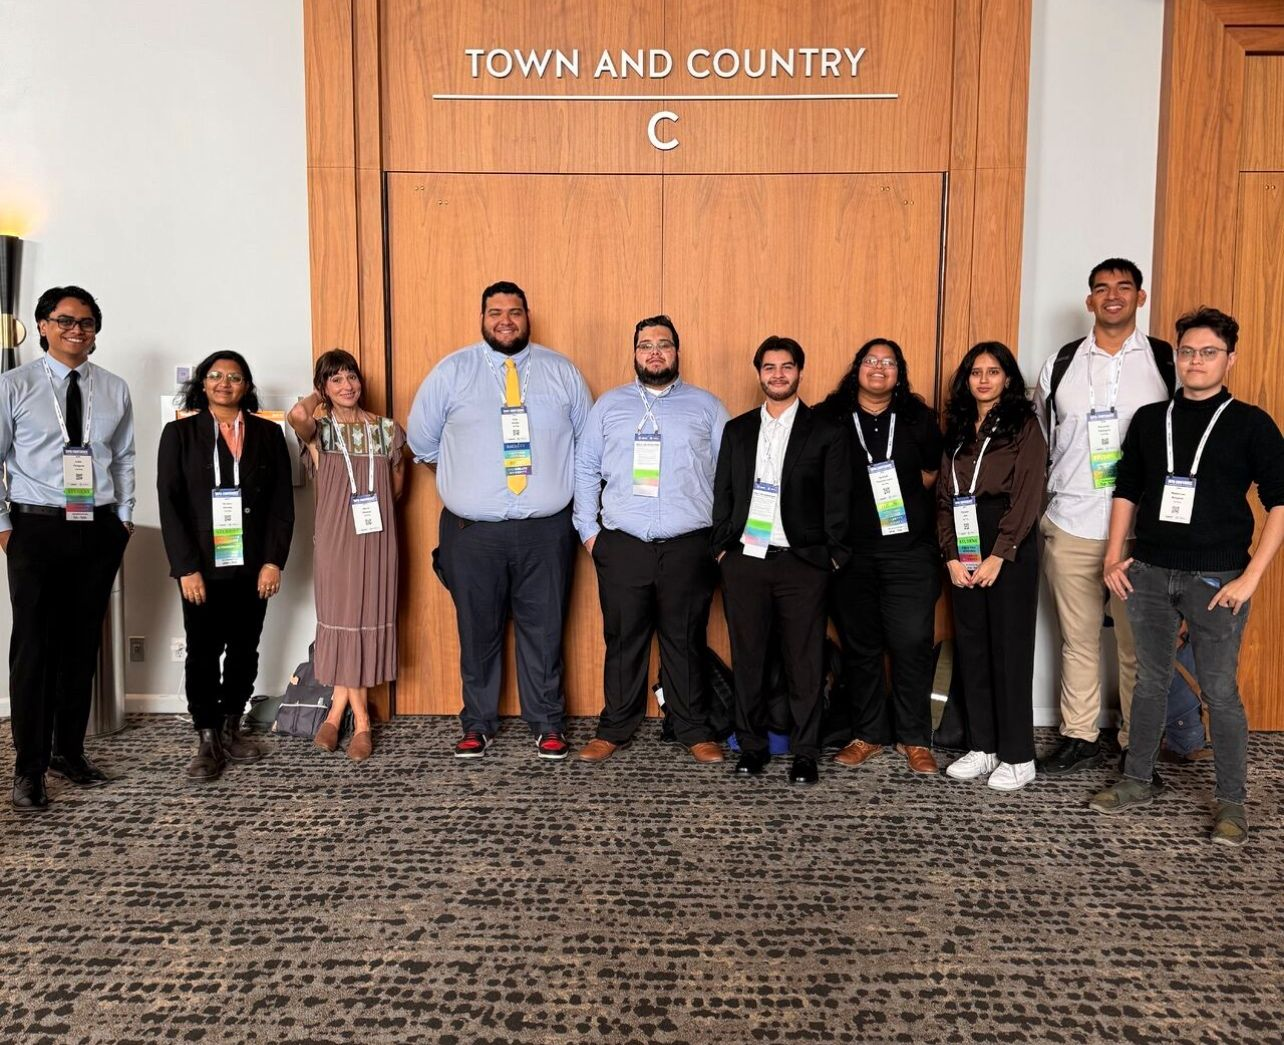
\includegraphics[width=\linewidth,height=2in,keepaspectratio]{welcome-group.png}
    \end{column}
  \end{columns}
\end{frame}

\begin{frame}{About Me}
  \begin{columns}[T,onlytextwidth]
    \begin{column}{0.54\textwidth}
      \begin{itemize}
        \item Full-Time Lecturer in Computer Science and Software Engineering.
        \item Teaching interests: introductory computing, data structures, object-oriented design, algorithms, and artificial intelligence.
        \item Research interests: deep reinforcement learning, heuristic search, robotics, and computer science education.
      \end{itemize}
    \end{column}
    \begin{column}{0.38\textwidth}
      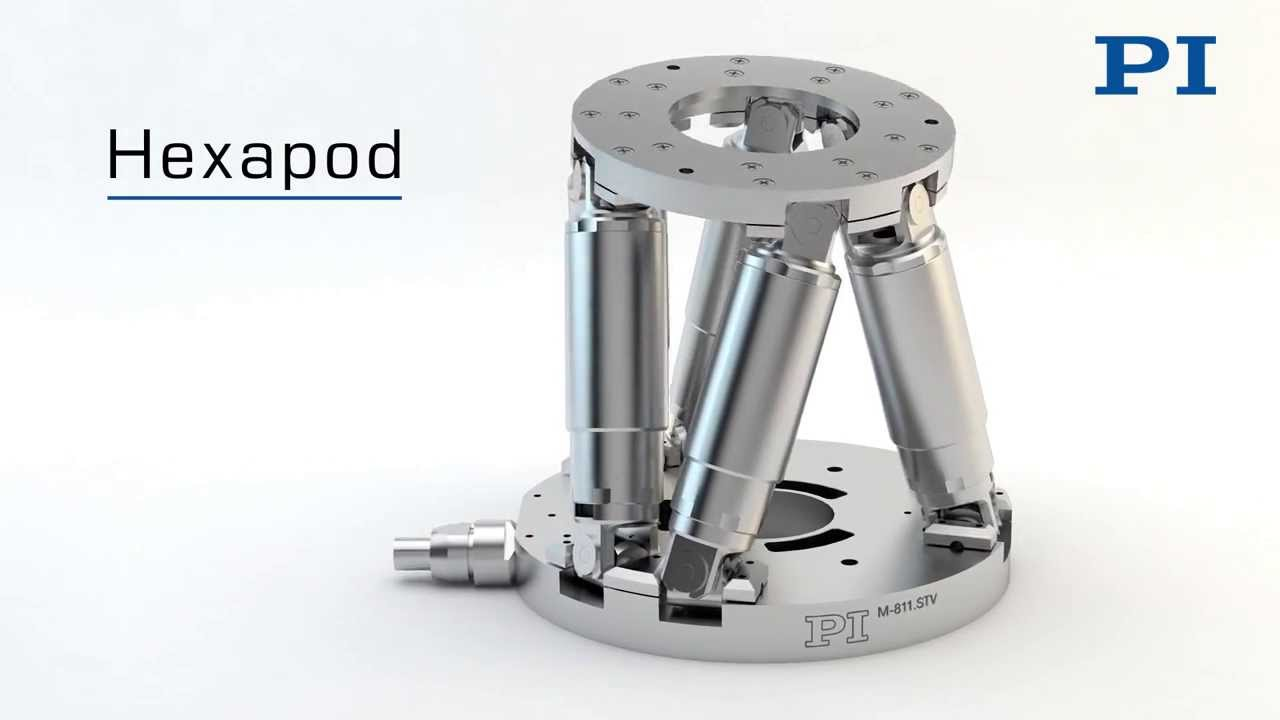
\includegraphics[width=\linewidth,height=2.25in,keepaspectratio]{about-research.png}
    \end{column}
  \end{columns}
\end{frame}

\begin{frame}{About Me: Path}
  \begin{itemize}
    \item Grew up in Boston.
    \item Went to high school in North Carolina.
    \item Started at community college in Los Angeles.
    \item Finished at UC Berkeley in applied mathematics and computer science.
    \item Earned an M.S. in computer engineering from Sonoma State.
    \item Spent time in doctoral study in computer science at UNH.
    \item Worked in Silicon Valley before coming to Cal Poly.
  \end{itemize}
\end{frame}

\begin{frame}[shrink=5]{About Me: Work And Life}
  \begin{columns}[T,onlytextwidth]
    \begin{column}{0.46\textwidth}
      \begin{block}{Professional}
        Robotics engineering at Physik Instrumente, machine learning engineering at Remi AI, and teaching/mentoring at Cal Poly.
      \end{block}
      \begin{block}{Mentoring}
        Beacons, OUDI, CENG SURP, projects, resumes, interview prep, and letters.
      \end{block}
    \end{column}
    \begin{column}{0.48\textwidth}
      \begin{center}
        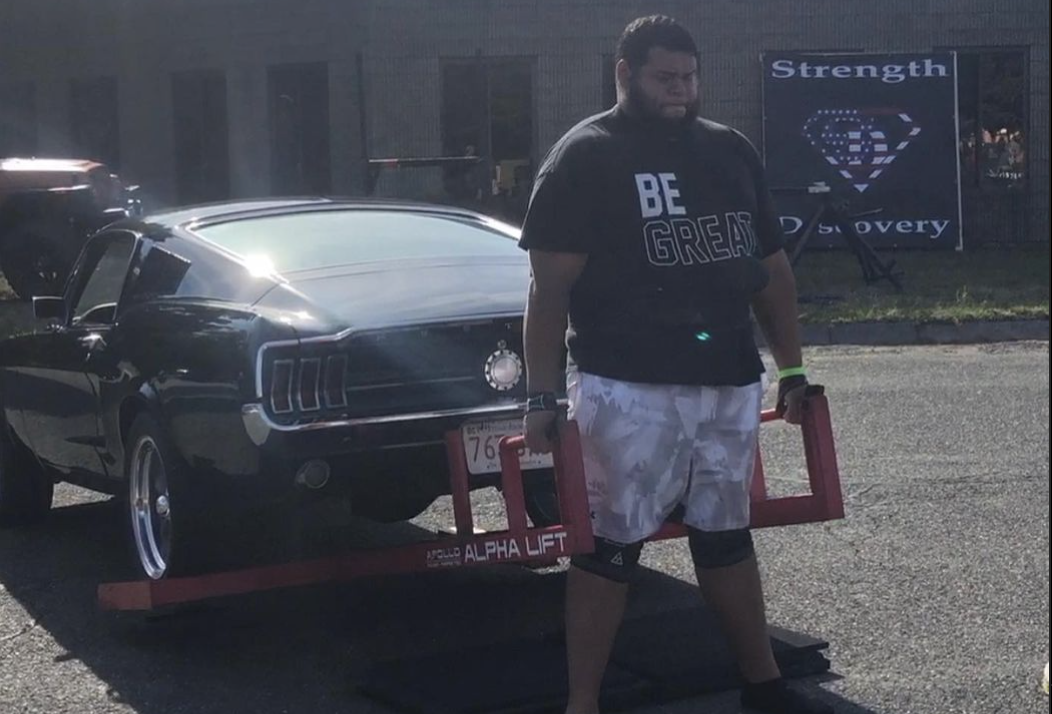
\includegraphics[width=0.48\linewidth,height=1.2in,keepaspectratio]{about-strongman.png}
        \hfill
        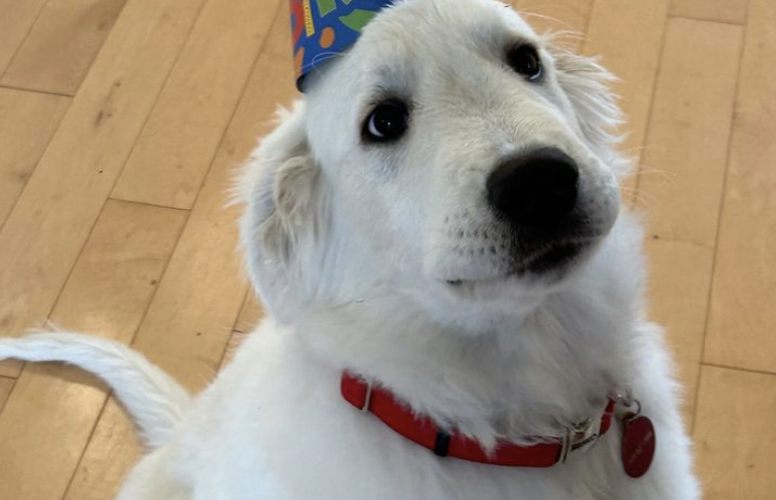
\includegraphics[width=0.48\linewidth,height=1.2in,keepaspectratio]{about-dog.png}
      \end{center}
      \begin{block}{Personal}
        Basketball, weightlifting, video games, anime, and trying to make technical ideas feel less mysterious. I am here to help you learn the material and navigate the field.
      \end{block}
    \end{column}
  \end{columns}
\end{frame}

\begin{frame}{Today}
  \begin{itemize}
    \item What computer science studies.
    \item Why computing exists as a discipline.
    \item Why computing matters even if you do not become a software engineer.
    \item How this course will work.
    \item What to set up before next time.
  \end{itemize}
\end{frame}

\sectionframe{Part 1: What Are We Studying?}

\begin{frame}{Computer Science}
  \begin{center}
    {\Huge What does this even mean?}
  \end{center}
\end{frame}

\begin{frame}{A Misleading Name}
  \begin{keyidea}
    ``Computer science'' can sound like the subject is mostly about computers.
  \end{keyidea}
  \vspace{0.12in}
  \begin{exampleblockcp}
    That is a little like calling mathematics ``calculator studies.''
  \end{exampleblockcp}
  \vspace{0.12in}
  \begin{itemize}
    \item Computers matter because they carry out computation.
    \item The deeper subject is how we represent problems and design precise processes.
  \end{itemize}
\end{frame}

\begin{frame}{Start With Computation}
  \begin{cpdefinition}
    Computation is the process of transforming information according to precise rules.
  \end{cpdefinition}
  \vspace{0.12in}
  \begin{exampleblockcp}
    A recipe, a payroll calculation, a route planner, a search engine, and a video game all describe processes over information.
  \end{exampleblockcp}
\end{frame}

\begin{frame}{Computer Science}
  \begin{cpdefinition}
    Computer science is the study of computation: how information can be represented, transformed, stored, communicated, and used to solve problems.
  \end{cpdefinition}
  \vspace{0.12in}
  \begin{itemize}
    \item A computer is one tool for carrying out computation.
    \item A program is a precise description of steps.
    \item A programming language gives us a way to write those steps for a machine and a human reader.
  \end{itemize}
\end{frame}

\begin{frame}{A Useful Mental Model}
  \begin{columns}[T,onlytextwidth]
    \begin{column}{0.3\textwidth}
      \begin{block}{Input}
        Data we start with.
      \end{block}
    \end{column}
    \begin{column}{0.3\textwidth}
      \begin{block}{Process}
        Rules we follow.
      \end{block}
    \end{column}
    \begin{column}{0.3\textwidth}
      \begin{block}{Output}
        Result we produce.
      \end{block}
    \end{column}
  \end{columns}
  \vspace{0.18in}
  \begin{activity}
    Pick one everyday task and identify its inputs, process, and outputs.
  \end{activity}
\end{frame}

\sectionframe{Part 2: Why Does Computer Science Exist?}

\begin{frame}{Why Does Computer Science Exist?}
  \begin{center}
    {\Huge Let's hear from you.}
  \end{center}
\end{frame}

\begin{frame}{Paper Work At Scale}
  \begin{columns}[T,onlytextwidth]
    \begin{column}{0.48\textwidth}
      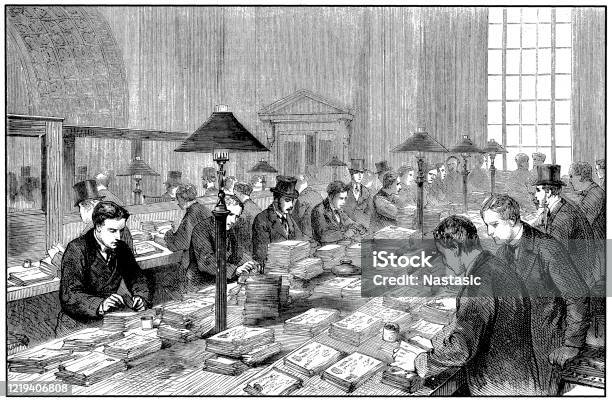
\includegraphics[width=\linewidth,height=1.5in,keepaspectratio]{bank-clerks.png}
    \end{column}
    \begin{column}{0.48\textwidth}
      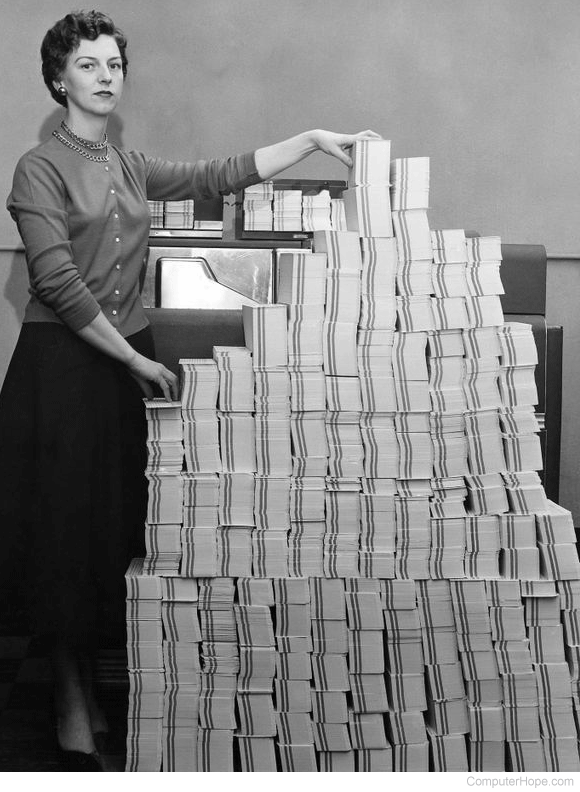
\includegraphics[width=\linewidth,height=1.5in,keepaspectratio]{punch-card-stack.png}
    \end{column}
  \end{columns}
  \vspace{0.08in}
  \begin{keyidea}
    A lot of early computing was about replacing or amplifying clerical labor: sorting, counting, tabulating, payroll, inventory, census work, and records.
  \end{keyidea}
\end{frame}

\begin{frame}{Drawing Work At Scale}
  \begin{columns}[T,onlytextwidth]
    \begin{column}{0.48\textwidth}
      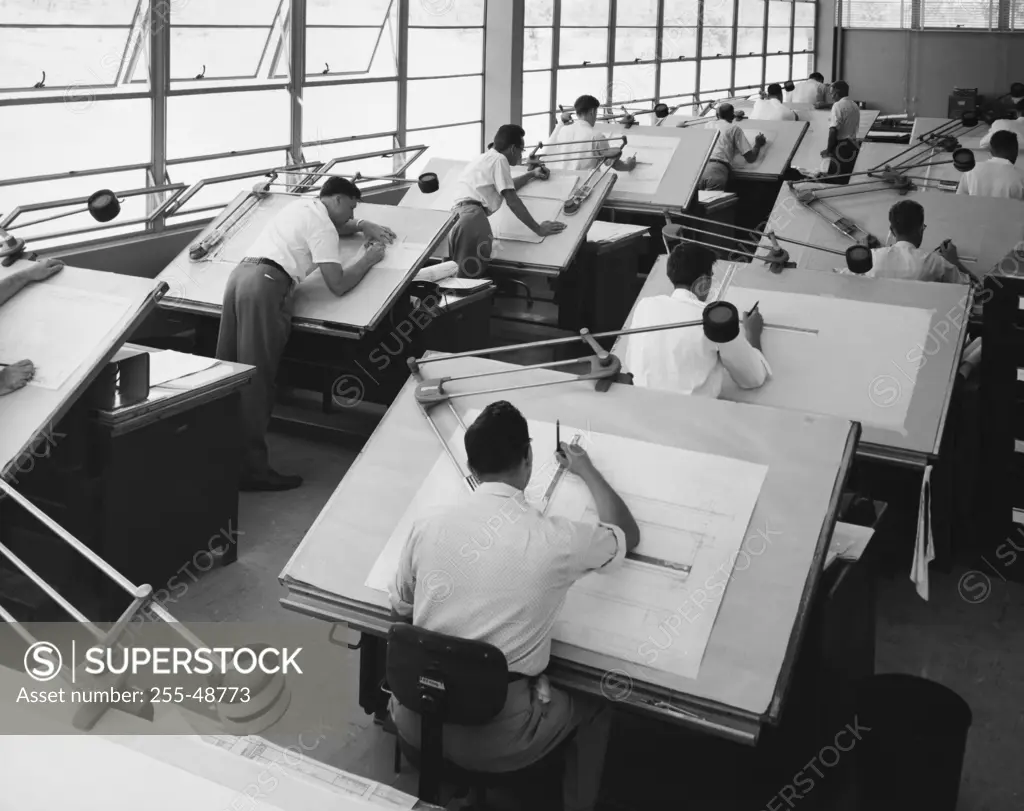
\includegraphics[width=\linewidth,height=1.5in,keepaspectratio]{drafting-engineers.png}
    \end{column}
    \begin{column}{0.48\textwidth}
      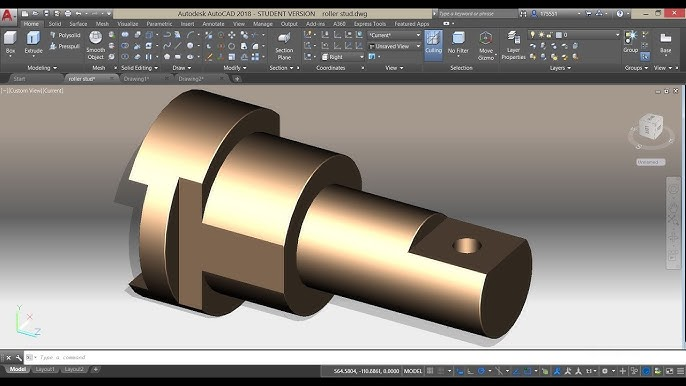
\includegraphics[width=\linewidth,height=1.5in,keepaspectratio]{cad-model.png}
    \end{column}
  \end{columns}
  \vspace{0.08in}
  \begin{keyidea}
    Computation turned drawings into editable, shareable models: design became something we could copy, simulate, revise, and manufacture from.
  \end{keyidea}
\end{frame}

\begin{frame}{Production Work At Scale}
  \begin{columns}[T,onlytextwidth]
    \begin{column}{0.48\textwidth}
      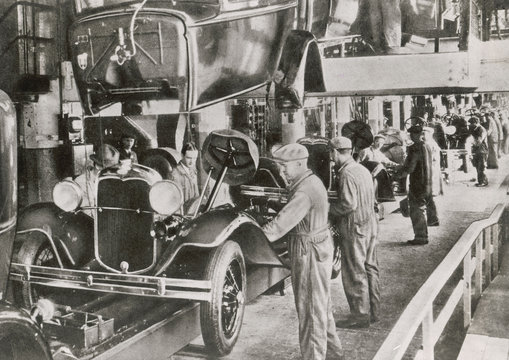
\includegraphics[width=\linewidth,height=1.5in,keepaspectratio]{assembly-line.png}
    \end{column}
    \begin{column}{0.48\textwidth}
      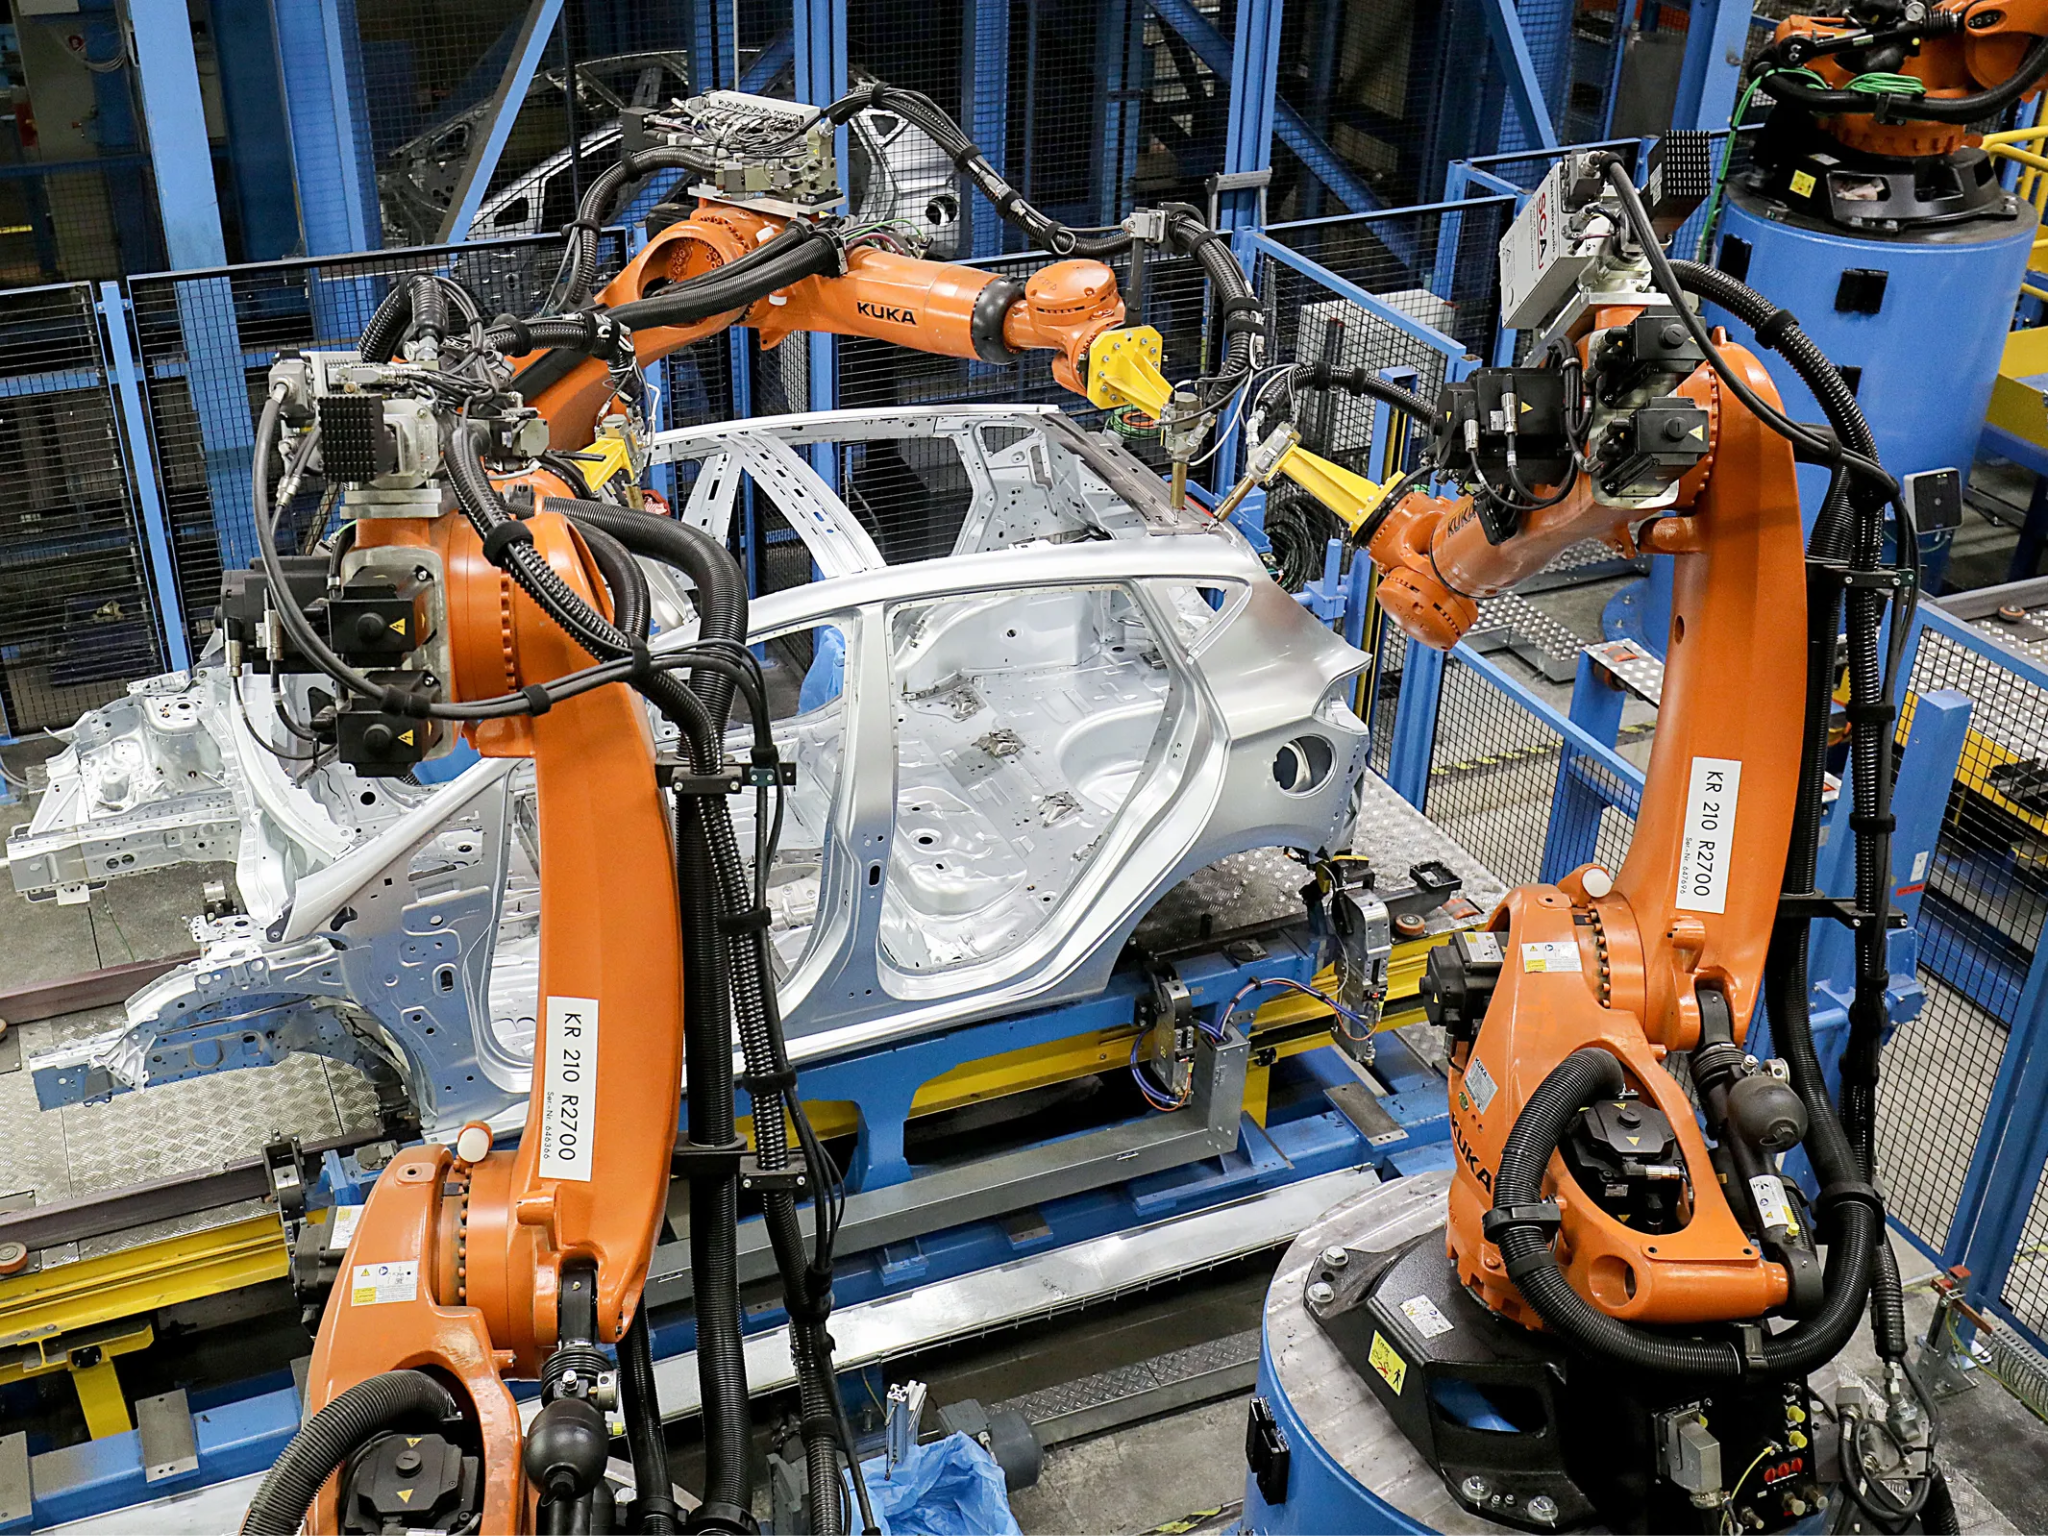
\includegraphics[width=\linewidth,height=1.5in,keepaspectratio]{robotic-assembly.png}
    \end{column}
  \end{columns}
  \vspace{0.08in}
  \begin{keyidea}
    Software does not only live on laptops. It coordinates machines, sensors, logistics, schedules, safety checks, and feedback loops.
  \end{keyidea}
\end{frame}

\begin{frame}{Everyday Models At Scale}
  \begin{columns}[T,onlytextwidth]
    \begin{column}{0.44\textwidth}
      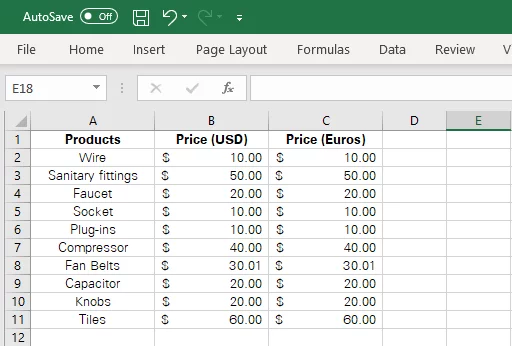
\includegraphics[width=\linewidth,height=2.2in,keepaspectratio]{spreadsheet.png}
    \end{column}
    \begin{column}{0.5\textwidth}
      \begin{keyidea}
        Spreadsheets made computation feel ordinary: not just for scientists, but for budgets, schedules, grades, inventory, experiments, and decisions.
      \end{keyidea}
      \begin{itemize}
        \item A table can become a model.
        \item A formula can become a rule.
        \item A change can ripple through a whole system.
      \end{itemize}
    \end{column}
  \end{columns}
\end{frame}

\begin{frame}{Reason 1: Scale}
  \begin{keyidea}
    Computers let us perform simple rules many times, quickly and consistently.
  \end{keyidea}
  \begin{itemize}
    \item Search millions of records.
    \item Simulate weather, traffic, or molecules.
    \item Coordinate communication across the world.
  \end{itemize}
\end{frame}

\begin{frame}{Reason 2: Precision}
  \begin{keyidea}
    Programming forces vague ideas to become precise procedures.
  \end{keyidea}
  \begin{exampleblockcp}
    ``Sort these names'' sounds simple until we ask: alphabetical by first name or last name? What about accents? What about ties? What about missing data?
  \end{exampleblockcp}
\end{frame}

\begin{frame}{Reason 3: Leverage}
  \begin{keyidea}
    A small program can affect a large number of people.
  \end{keyidea}
  \begin{itemize}
    \item That can be wonderful: accessibility tools, medical analysis, education, art.
    \item That can be dangerous: bias, privacy failures, brittle automation.
    \item This is why we practice both technical care and social responsibility.
  \end{itemize}
\end{frame}

\begin{frame}[shrink=4]{Economic Impact}
  \begin{keyidea}
    Each wave of computing turned a technical idea into a new economic platform.
  \end{keyidea}
  \begin{columns}[T,onlytextwidth]
    \begin{column}{0.46\textwidth}
      \begin{block}{Long arc}
        Mainframes, personal computers, the web, mobile/cloud, and now AI all changed what firms can measure, automate, sell, and scale.
      \end{block}
    \end{column}
    \begin{column}{0.48\textwidth}
      \begin{block}{Current scale}
        BEA estimated that digital economy real value added grew 6.3\% in 2022, compared with 1.9\% for total U.S. real GDP.
      \end{block}
      \begin{block}{Public markets}
        S\&P lists Information Technology at 36.8\% of the S\&P 500 by index weight as of July 31, 2026.
      \end{block}
    \end{column}
  \end{columns}
\end{frame}

\begin{frame}{The Impact Of Computer Science}
  \begin{activity}
    Think of one system you used this week that made a decision about you, for you, or near you.
  \end{activity}
  \vspace{0.12in}
  \begin{itemize}
    \item What information did it use?
    \item What did it output?
    \item Who benefited?
    \item Who could be harmed if it failed?
  \end{itemize}
\end{frame}

\begin{frame}{The Point}
  \begin{keyidea}
    Computer science is not only about computers. It is about building precise tools for messy human problems.
  \end{keyidea}
  \vspace{0.12in}
  \begin{itemize}
    \item We need logic.
    \item We need creativity.
    \item We need communication.
    \item We need judgment.
  \end{itemize}
\end{frame}

\sectionframe{Part 3: Why Study Computer Science?}

\begin{frame}{Why Study Computer Science?}
  \begin{center}
    {\Huge Let's hear from around the room.}
  \end{center}
\end{frame}

\begin{frame}{A Practical Answer}
  \begin{itemize}
    \item Computing is part of nearly every discipline.
    \item Programming helps you automate work and analyze information.
    \item Reading code helps you understand the systems around you.
    \item Debugging builds a general problem-solving muscle.
  \end{itemize}
\end{frame}

\begin{frame}{A Deeper Answer}
  \begin{keyidea}
    You are learning a new way to think: break a problem into pieces, make assumptions explicit, test your reasoning, and revise.
  \end{keyidea}
  \vspace{0.12in}
  \begin{exampleblockcp}
    This way of thinking transfers beyond Python: spreadsheets, data analysis, research, design, engineering, operations, and everyday troubleshooting.
  \end{exampleblockcp}
\end{frame}

\begin{frame}{Who Counts As A Computer Scientist?}
  \begin{keyidea}
    The people who shaped computing do not all fit one narrow stereotype.
  \end{keyidea}
  \vspace{0.02in}
  \portraitcard{gh.jpg}{Grace Hopper}{Navy officer, compiler pioneer; made programming more usable.}
  \hfill
  \portraitcard{kj.jpeg}{Katherine Johnson}{NASA mathematician and ``human computer'' for spaceflight.}
  \hfill
  \portraitcard{rt.jpg}{Richard Tapia}{First-generation Mexican American mathematician; optimization and mentoring.}
  \hfill
  \portraitcard{at.jpg}{Alan Turing}{Mathematician/logician; theory, cryptanalysis, and machines.}
\end{frame}

\begin{frame}{Why These Examples Matter}
  \begin{exampleblockcp}
    They seem ``nontraditional'' only if the stereotype is too narrow.
  \end{exampleblockcp}
  \vspace{0.06in}
  \begin{itemize}
    \item Hopper: Navy officer who argued programming should be closer to human language.
    \item Johnson: mathematical labor before electronic machines took over much of that work.
    \item Tapia: first-generation path and mentoring that widened who belongs.
    \item Turing: logic and mathematics before ``software engineer'' was a job title.
  \end{itemize}
\end{frame}

\begin{frame}{Belonging In Computer Science}
  \begin{keyidea}
    Maybe the problem is not that students fail to match the ``traditional'' CS type. Maybe the stereotype is wrong.
  \end{keyidea}
  \vspace{0.12in}
  \begin{itemize}
    \item Computing has always been built by people with different paths, skills, identities, and motivations.
    \item The useful question is not ``Do I look like a computer scientist?''
    \item The useful question is ``What problems can I learn to reason about?''
  \end{itemize}
\end{frame}

\begin{frame}{Community}
  \begin{columns}[T,onlytextwidth]
    \begin{column}{0.34\textwidth}
      
\includegraphics[width=\linewidth,height=2.25in,keepaspectratio]{colorstack.png}
    \end{column}
    \begin{column}{0.58\textwidth}
      \begin{block}{Color Coded by ColorStack}
        Cal Poly has a supportive community for students interested in computing, belonging, professional development, and peer support.
      \end{block}
      \begin{itemize}
        \item Join the Discord.
        \item Watch for events and resources.
        \item Bring a friend.
      \end{itemize}
    \end{column}
  \end{columns}
\end{frame}

\sectionframe{Part 4: How This Course Works}

\begin{frame}{What We Practice In CS 1001}
  \begin{itemize}
    \item Reading code carefully.
    \item Predicting what a program will do before running it.
    \item Writing small programs that solve clear problems.
    \item Testing, debugging, and explaining your reasoning.
  \end{itemize}
  \vspace{0.15in}
  \begin{keyidea}
    The goal is not memorizing Python syntax. The goal is building a durable way to think.
  \end{keyidea}
\end{frame}

\begin{frame}{How The Course Will Feel}
  \begin{columns}[T,onlytextwidth]
    \begin{column}{0.48\textwidth}
      \begin{block}{Early weeks}
        Expressions, variables, functions, conditionals, and tracing.
      \end{block}
      \begin{block}{Middle weeks}
        Lists, strings, mutation, loops, dictionaries, and structured data.
      \end{block}
    \end{column}
    \begin{column}{0.48\textwidth}
      \begin{block}{Later weeks}
        Objects, algorithms, files, larger programs, and applications.
      \end{block}
      \begin{block}{All quarter}
        Practice, feedback, persistence, and small wins that compound.
      \end{block}
    \end{column}
  \end{columns}
\end{frame}

\begin{frame}{The Reality Check}
  \begin{itemize}
    \item We start slowly on purpose.
    \item The pace will increase as ideas combine.
    \item The hard part is usually not typing code; it is reasoning about state, order, and edge cases.
    \item Waiting until the night before makes programming feel much harder than it needs to.
  \end{itemize}
  \vspace{0.12in}
  \begin{activity}
    The move: start early, get stuck early, ask early.
  \end{activity}
\end{frame}

\begin{frame}{Student Expectations}
  \begin{block}{Math}
    Comfort with arithmetic and basic algebra helps with calculations, variables, and logical structure.
  \end{block}
  \begin{block}{Attention to detail}
    Small differences matter: names, parentheses, indentation, punctuation, and order.
  \end{block}
  \begin{block}{Communication}
    You will explain what your code does and why it works.
  \end{block}
\end{frame}

\begin{frame}{More Expectations}
  \begin{block}{Problem solving}
    Break tasks into steps, test assumptions, and revise your plan when reality disagrees.
  \end{block}
  \begin{block}{Time management}
    Programming rewards steady practice. Short repeated sessions beat heroic last-minute sessions.
  \end{block}
  \begin{block}{Persistence}
    Confusion is not failure. It is the normal starting point for learning a technical skill.
  \end{block}
\end{frame}

\begin{frame}{Canvas And Course Materials}
  \begin{itemize}
    \item Canvas will host announcements, assignments, grades, and due dates.
    \item Public slides will also be available from the course website.
    \item Example code will be posted when it helps you practice.
  \end{itemize}
  \vspace{0.18in}
  \begin{activity}
    Open Canvas, find this course, find today's lecture slides, and open the syllabus.
  \end{activity}
\end{frame}

\sectionframe{Part 5: First Technical Setup}

\begin{frame}{Technical Skill: Search}
  \begin{keyidea}
    Being able to search well is part of being able to program well.
  \end{keyidea}
  \begin{enumerate}
    \item Search for Google Colab.
    \item Open a new notebook.
    \item Search for how to print \texttt{Hello, world!} in Python.
  \end{enumerate}
\end{frame}

\begin{frame}{Technical Skill: Typing}
  \begin{itemize}
    \item Comfortable typing makes practice less frustrating.
    \item You do not need to be fast today.
    \item Accuracy matters more than speed.
  \end{itemize}
  \vspace{0.15in}
  \begin{exampleblockcp}
    Optional practice site: \texttt{https://monkeytype.com/}
  \end{exampleblockcp}
\end{frame}

\begin{frame}{Technical Skill: Copy, Paste, Run}
  \begin{enumerate}
    \item Copy a small Python \texttt{Hello, world!} example.
    \item Paste it into your Colab notebook.
    \item Click the run button.
    \item Change the message and run it again.
  \end{enumerate}
  \vspace{0.12in}
  \begin{keyidea}
    Running code is a conversation with the machine. Change one thing, observe what changes.
  \end{keyidea}
\end{frame}

\begin{frame}{Technical Skill: File Management}
  \begin{enumerate}
    \item Create a folder somewhere on your computer.
    \item Give it a boring, obvious name: \texttt{CS1001}, \texttt{Fall\_CS1001}, or \texttt{IntroComputing}.
    \item Save your first notebook or file there.
    \item Make sure you can find it again.
  \end{enumerate}
\end{frame}

\sectionframe{Part 6: The Sales Pitch}

\begin{frame}{My Commitment: Beyond Syntax}
  \begin{itemize}
    \item We are not just memorizing Python.
    \item We are learning the underlying mechanisms of computing.
    \item By the end, you should have logic that transfers to other languages and tools.
    \item This course is foundation for future computing work.
  \end{itemize}
\end{frame}

\begin{frame}{The Scientist's Mindset}
  \begin{itemize}
    \item I will ask you questions.
    \item It is okay to say ``I do not know.''
    \item Our job is not to know instantly.
    \item Our job is to figure things out carefully.
  \end{itemize}
  \vspace{0.15in}
  \begin{activity}
    When you get stuck, say what you expected, what happened, and what you tried.
  \end{activity}
\end{frame}

\begin{frame}{Before Next Time}
  \begin{itemize}
    \item Read the syllabus.
    \item Make sure you can access Canvas.
    \item Create your course folder.
    \item Run \texttt{print("Hello, world!")} in Python.
    \item Bring one question about computers, programs, or the course.
  \end{itemize}
  \vspace{0.18in}
  \begin{keyidea}
    Next time: how computers execute programs.
  \end{keyidea}
\end{frame}

\begin{frame}{Next Time}
  \begin{center}
    {\Huge How Computers Execute Programs}
  \end{center}
\end{frame}

\end{document}
